\documentclass{fithesis}

\usepackage{listings}
\usepackage{lmodern}
\usepackage[czech]{babel}
\usepackage[utf8]{inputenc}
\usepackage{cmap}
\usepackage{graphicx}
\usepackage[T1]{fontenc} %formátuje české znaky - důležité
\usepackage[plainpages=false, pdfpagelabels]{hyperref}
\usepackage{hyperref}
%\usepackage{makeidx}
%\makeindex
\def\figureautorefname{Obrázek}%
\def\tableautorefname{Tabulka}%

%\bibliographystyle{unsrt}


%\makeindex
\thesistitle{Integrace DMS a workflow v Liferay Portal}
\thesissubtitle{Diplomová práce}
\thesisstudent{Marek Tlačbaba}
\thesiswoman{false}
\thesisfaculty{fi}
\thesisyear{2014}
\thesisadvisor{RNDr. Jaroslav Ráček, Ph.D.}


\begin{document}

\FrontMatter
\ThesisTitlePage

\begin{ThesisDeclaration}
Prohlášení\AdvisorName
\end{ThesisDeclaration}

\begin{ThesisThanks}
Poděkování
\end{ThesisThanks}

\begin{ThesisAbstract}
Shrnutí
\end{ThesisAbstract}

\begin{ThesisKeyWords}
Klíčová slova
\end{ThesisKeyWords}


\MainMatter
\setcounter{secnumdepth}{4}
\tableofcontents

\chapter*{Úvod}
\addcontentsline{toc}{chapter}{Úvod}


\chapter{Podnikové portály}

Pojem portál bývá definován různými způsoby v závislosti na situaci, ve které je používán. Dříve se portály zaměřovaly na jednotný přístup k informacím nezávisle na jejich původu a umístění. S~dalším vývojem informačních technologií se postupně tento přístup rozšiřoval a~do definice portálu přibyly pojmy jako integrace a agregace služeb a aplikací. V následujícím textu je uvedeno několik definic portálu a podnikového portálu.

Například Gála definoval portál jako jednotné rozhraní, ve kterém lze pracovat s běžnými službami a nástroji jako jsou, například zpravodajství a~komunikace, mimo to je v něm zaručen přístup k všeobecným aplikacím jako jsou vlastní stránky a blogy, a k aplikacím specializovaným, například slovníkům. \cite{gala}

Další definice portálu je převzata ze standardu JSR-286 a zní následovně: Portál je webová aplikace, která (obvykle) poskytuje možnost personalizace, autentifikace, agregace obsahu z různých zdrojů a slouží jako prezentační vrstva informačních systémů. Agregací se rozumí integrace obsahu z různých zdrojů v rámci jedné webové stránky. Portál může mít vysoce propracované nástroje pro personalizaci, které poskytují obsah upravitelný podle přání uživatele. Stránky portálu mohou mít různé skupiny portletů \footnote[1]{Bližší informace v dalších částech této práce.}, které vytvářejí obsah pro různé uživatele.  \cite{jsr-286}

Předchozí definice se týkají portálu obecně, proto zde uvedu také definici podnikového portálu jako takového. Například podle Čecha je podnikový portál definován jako internetové nebo intranetové stránky, které slouží jako vstupní bod, respektive brána k různým datovým, informačním a znalostním zdrojům v organizaci. Jejich cílem je zpřístupnit tyto zdroje specifické skupině lidí. Může to být jak zákazníkům, tak také vlastním zaměstnancům nebo partnerům. \cite{cech}

V předchozích definicích portálu jsou naznačeny některé základní rysy podnikových portálů. Mezi důležité vlastnosti můžeme považovat jediný přístupový bod, integrace, federace, přizpůsobivost, personalizace, kontrola přístupu a vyhledávání v podnikovém obsahu, tak jak jsou uvedeny v \cite{enterprise-portal}.

\section{Konkrétní portálová řešení}
Existuje a používá se celá řada konkrétních portálových řešení. Nejčastěji bývají implementovány v jazyce Java a podporují standardy JSR-168 a JSR-286 \footnote[2]{Bližší informace v dalších částech této práce} pro tvorbu portletů v jazyce Java. Existují také portály i pro jiné technologie, například pro platformu .NET je možné využít Microsoft SharePoint, ale nejvíce řešení existuje pro jazyk Java, kde mezi nejznámější patří IBM Websphere Portal, JBoss GateIn, Oracle WebCenter či Liferay Portal. Tyto portály již většinou obsahují velké množství připravených portletů, např. wiki stránky, správu souborů, portlety pro komunikaci a další.

\section{Liferay Portal}
Liferay Portal je open source podnikový portál založený na jazyce Java vyvíjený společností Liferay, Inc.. Podporuje specifikace JSR-168 a JSR-286 pro tvorbu portletů v jazyce Java. Liferay Portal je k dispozici ve dvou edicích, Community Edition (CE) a Enterprise Edition (EE).

Liferay Portal CE je bezplatná verze portálu, která je volně dostupná ke stažení. Tato verze neobsahuje oficiální podpory, je zde pouze podpora poskytovaná prostřednictvím Liferay komunity. Druhá verze portálu, Liferay Portal EE, je placená edice. U této verze je kladen velký důraz na stabilitu, bezpečnost a výkon. K této edici patří dlouhodobá podpora od společnosti Liferay, Inc. nebo jejích oficiálních partnerů.

Ihned po instalaci portálu je k dispozici množství již předinstalovaných portletů. Je možné například okamžitě využívat wiki stránky, fórum, kalendář či galerii obrázků. Liferay Portal podporuje různé způsoby úprav či rozšíření. Pro změny vzhledu můžeme využít témata či šablony, další funkcionalitu portálu je možno přidávat pomocí portletů. Pro změnu portálu či portletů se používají tzv. hooks. Pokud se jedná o větší a zásadnější změny přímo v jádru portálu, ty se provádí pomocí pluginu Ext. \cite{developer-guide}

Portál Liferay nabízí svým uživatelům zabezpečené jednotné přihlášení, nástroje pro správu workflow, snadnou instalaci samotného portálu i dalších nových aplikací a rozšíření. Od verze 6.1 CE GA2 umožňuje instalaci rozšíření a aplikací nově také z Liferay Marketplace. Takto je možné stahovat aplikace přímo z rozhraní portálu a jednoduše je přidat do portálu.

Liferay také obsahuje pokročilý systém pro správu obsahu (Liferay CMS), který umožňuje oprávněným uživatelům vytvářet a spravovat obsah webu přímo z prohlížeče a to i bez znalosti programování. S tím také souvisí možnost dělit uživatele do organizací, skupin a uživatelům přidělovat role, podle kterých jim následně zobrazovat různý obsah, aplikace a umožňovat provádět různé akce.

Mezi další vlastnosti portálu patří vícejazyčné uživatelské rozhraní, personalizace portálových stránek, jednoduchá úprava stránek způsobem táhni a pusť, automatické nahrávání souborů.

Liferay také podporuje různé platformy a proto je možné ho provozovat na různých aplikačních serverech, operačních systémech a databázích. Také podporuje různé metody integrace včetně SOAP, REST, RSS a také další proprietární rozhraní.\cite{liferay-features}

To jsou některé z důvodů, proč se podnikový portál Liferay stal rozšířenou a oblíbenou platformou pro vývoj firemních webů a systému v jazyce Java.


\chapter{Vývoj portletů}
V této kapitole bude popsán vývoj portletů, které tvoří obsah portálů.

\section{Portlet}
Portlet je webová aplikace, která poskytuje uživatelům specifický obsah, typicky informaci nebo službu. Portlet je spravován portletovým kontejnerem, který zpracovává požadavky portletu a následně generuje dynamický obsah v podobě fragmentů v některém ze značkovacích jazyků -- HTML, XHTML, WML. Tyto fragmenty jsou pak spojovány a dohromady vytváří portálovou stránku.

Portletový kontejner má tedy odpovědnost za řízení životního cyklu jednotlivých portletů a je v něm také uloženo nastavení uživatele pro daný portlet. Ale části generované jednotlivými portlety slučuje dohromady na stránku portál. Portál a portletový kontejner mohou být postaveny jako jedna komponenta ale mohou to být také komponenty dvě. Na následujícím obrázku 3.1 je zobrazen průběh vytváření stránky v portálu tak, jak bylo výše naznačeno.

\begin{figure}[htp]
\centering
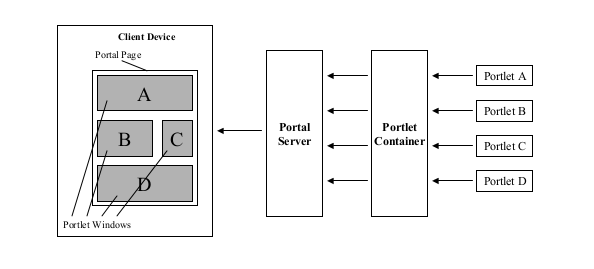
\includegraphics[width=340px]{images/vytvareni_stranky_v_portalu.png}
\caption{Vytváření stránky v portálu (převzato z \cite{jsr-286})}
\end{figure}

\section{Specifikace}
Důvodem pro vytvoření portletové specifikace byla situace, kdy různí dodavatelé používali svá vlastní API, která neumožňovala přenositelnost mezi portálovými servery.

První verze Java Portlet Specification 1.0 (JSR-168) byla vydána v roce 2003. V této specifikaci ještě bylo stále různé nedostatky a chyby, které pak tvůrci portletů stejně řešili každý po svém. To způsobovalo i nadále, že portlety byly mezi portálovými servery stále problematicky přenositelné či nepřenositelné úplně. Proto vznikla druhá verze Java Portlet Specification 2.0 (JSR-286) a ta byla vydána v červnu 2008. Mezi nejdůležitější přínosy patří následující:
\begin{itemize}
\item sdílení parametrů mezi portlety skrz veřejné render parametry,
\item meziportletová komunikace pomocí zasílaní událostí,
\item transformace informací nově definovanými portletovými filtry,
\item možnost portletů poskytovat zdroje jako jsou například PDF soubory.
\end{itemize}
Většina portletových kontejnerů sice poskytuje k základním požadavkům i svá rozšíření. Tyto rozšíření však nemusíme využívat a tak můžeme zachovat myšlenku snadné přenositelnosti.

\subsection{Životní cyklus portletu}
Každý portlet musí implementovat rozhraní \verb|Portlet|. Toto rozhraní obsahuje čtyři základní metody, které musí být implementovány a které řídí životní cyklus portletu - \verb|init(), processAction(), render(), destroy()|.

Metoda \verb|init()| je volána ihned při vytváření portletu a je používána například pro přípravu zdrojů potřebných portletem.

Metoda \verb|processAction()| je volána vždy po provedení nějaké akce uživatelem, když se touto akcí nějak mění stav portletu. Může to být například akce potvrzení formuláře a následné zpracování a uložení dat v databázi.

Metoda \verb|render()| má za úkol generovat fragment stránky, který je pak dostupný uživateli v portletu. V této metodě by se neměl měnit stav portletu.

Poslední metodou je \verb|destroy()|. Ta je volána před odstraněním portletu z paměti. Poskytuje poslední možnost pro uvolnění zdrojů, které byly portletem používány. \cite{jsr-286}

Zpracování požadavků v portletech může procházet několika fázemi zpracování.

\begin{itemize}
\item Render -- vykreslovací fáze, ve které se typicky nemění stav portletu, odpovídá jí metoda \verb|render()|.
\item Action -- portlet zpracovává nějakou akci a typicky mění svůj stav, odpovídá ji metoda \verb|processAction()|.
\item Resource -- portletem je poskytován nějaký zdroj, např. PDF soubory. Aby portlet mohl podporovat tuto funkcionalitu, musí implementovat rozhraní \verb|ResourceServingPortlet|.
\item Event -- portlet přijímá nějakou událost a nějak na ni reaguje. Portlet v tomto případě musí implementovat rozhraní \verb|EventPortlet|.
\end{itemize}

Všechny tyto rozhraní implementuje abstraktní třída \verb|GenericPortlet|. Tato třída obsahuje implementaci všech povinných metoda a několika dalších, které je možné využít.

Po každé action fázi musí následovat fáze render. Pokud se na portálové stránce vyskytuje více portletů, je metoda render zavolána u všech zobrazených portletů. 

\subsection{Režimy portletu}
Portletová specifikace obsahuje tři režimy portletu, které umožňují zobrazit jiný obsah v závislosti na požadovaném úkolu. Tyto režimy využívá metoda \verb|render()|, která podle nich vygeneruje odpovídající obsah.

\begin{itemize}
\item View -- základní režim používaný při klasickém zobrazení portletu na portálové stránce.
\item Edit -- nepovinný, uživateli umožňuje nastavovat portlet.
\item Help -- nepovinný, zobrazuje se nápověda k danému portletu.
\end{itemize}

Ve třídě \verb|GenericPortlet| jsou k těmto účelům definovány metody \verb|doView()|, \verb|doEdit()| a \verb|doHelp()|. Jednotlivé portletové režimy by měli být implementovány přetížením těchto metod. Každý portál si také může definovat vlastní portletové režimy. Každý portlet musí mít zadefinováno, které režimy podporuje.

\subsection{Stavy okna}
Portletová specifikace definuje tři základní stavy.

\begin{itemize}
\item Minimized -- okno portletu je minimalizované.
\item Normal -- původní velikost portletu, které umožňuje zobrazení všech portletů na na portálové stránce.
\item Maximized -- okno portletu skryje ostatní portlety na stránce a zobrazuje se pouze tento maximalizovaný portlet, nebo zakrývá většinu dostupné plochy.
\end{itemize}

\subsection{Struktura portálové aplikace}
Portálové aplikace jsou uloženy ve standardní archivním souboru jazyka Java, Web ARchive (WAR). Mohou obsahovat více portletů, servlety, JSP soubory a další. Musí obsahovat webový deskriptor a také navíc portletový deskriptor implementace \verb|portlet.xml|.


















\chapter{Workflow}
Jednoznačná definice workflow neexistuje, jelikož každá oblast, ve které je workflow používáno, si ho definuje po svém. Obecně je ale možné definovat workflow jako proces automatizace podnikových procesů. O sjednocení této terminologie se již v roce 1996 pokusila institut Workflow Management Coalition (WfMC), kdy vydal terminologický slovník, ve kterém je workflow definováno takto: 

Workflow znamená automatizaci celého nebo části podnikového procesu, během kterého jsou dokumenty, informace nebo úkoly předávány od jednoho účastníka procesu k druhému podle sady procedurálních pravidel tak, aby se dosáhlo nebo přispělo k plnění celkových/globálních podnikových cílů. \cite{wfmc}

V počítačových systémech je workflow definováno jako systém řízení workflow. V tomto systému je možné workflow definovat, vytvořit a celý průběh procesu řídit. Mezi jeho úkoly patří provádět definici procesu, komunikovat s účastníky workflow, případně spouštět další aplikace nutné k vykonání workflow.


\section{Typy workflow systému}
Workflow systémy se mohou dělit do několika skupin podle různých hledisek či typů. \cite{workflow}

\subsection{Hledisko charakteru procesů}
\begin{itemize}
\item \textbf{Administrativní} workflow systémy jsou určeny k vyřizování běžných administrativních úkonů, které jsou většinou jednoduché, opakující se a dobře strukturované.
\item \textbf{Ad-hoc} workflow systémy jsou založeny na náhodnosti vzniku. Procesy bývají jedinečné a je nutné je definovat až při jejich vzniku.
\item \textbf{Kolaborativní} workflow systémy podporují především týmovou spolupráci. Zde je typickým znakem existence nějakého dokumentu, skrze který si uživatelé vyměňují poznatky a většinou se tento dokument stává i výsledkem společné práce. Často obsahuje opakovaní několika iterací stejného kroku dokud nedojde ke shodě.
\item \textbf{Produkční} workflow systémy podporují hlavní podnikové procesy, které vytvářejí přidanou hodnotu k finálnímu produktu.
\end{itemize}

\subsection{Hledisko orientace procesů}
\begin{itemize}
\item \textbf{Procesy orientované na lidi.} U těchto systémů spoléhají účastníci sami na sebe. Předávané informace jsou proměnlivé a procesy nejednotné a špatně předpověditelné. Z těchto důvodů jsou průběhy závislé na jednotlivcích.
\item \textbf{Procesy orientované na sebe.} Tyto systémy jsou zaměřené na klíčové procesy, které obvykle bývají hlavními aktivitami podniku. Jejich pravidla řešení a jejich zpracování jsou pevně daná.
\end{itemize}

\subsection{Hledisko technologické infrastruktury}
Podle technologické infrastruktury, nad kterou je systém workflow postaven, lze produkty rozdělit do několika skupin.
\begin{itemize}
\item Založené na \textbf{elektronické poště} -- využívají dostupné emailové servery. Uživatelé nepotřebují speciální software.
\item Založené na \textbf{procesech} -- mohou implementovat vlastní komunikační mechanismus a jsou postaveny na určitém databázovém systému. Bývají tvořeny jako komplexní řešení uceleného konceptu workflow.
\item Založené na \textbf{webu} -- využívají jednotného rozhraní intranetové aplikace. Je to univerzální platforma pro sdílení informací.
\item Založené na \textbf{dokumentech} -- tyto systémy byly motivovány představou o směrování dokumentů. Využívají systémy pro správu dokumentů.
\end{itemize}

\section{Obecný model workflow systému}
Institut WfMC vytvořil obecný model, kde mají produkty podobné komponenty viz obr. 4.1. Jednotlivé komponenty systému se dělí na programové a datové.

\begin{figure}[htp]
\centering
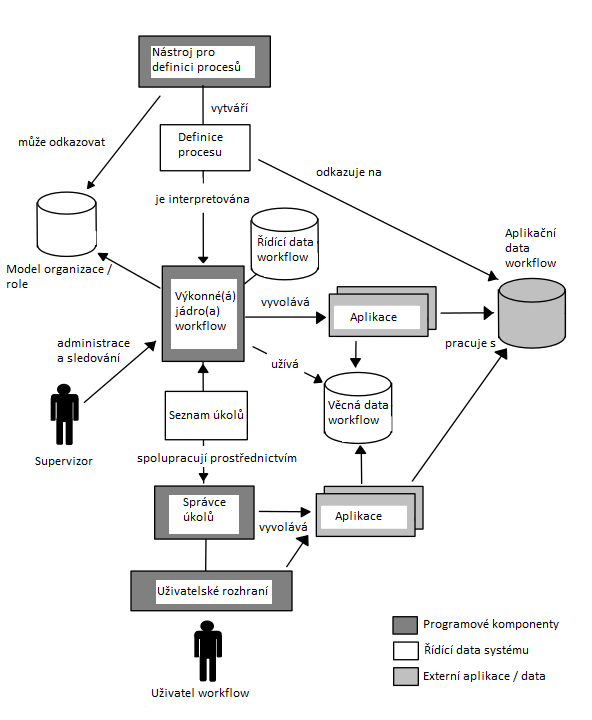
\includegraphics[width=340px]{images/obecny_model.png}
\caption{Obecný model workflow (převzato z \cite{wfmc})}
\end{figure}

Programové komponenty.

\begin{itemize}
\item Nástroj pro definici procesů (definition tool) umožňuje definovat procesy, přiřazovat role a stanovat pravidla.
\item Výkonné jádro workflow (workflow engine) řídí průběh workflow procesů, spouští nutné externí aplikace a udržuje statistiky o průběhu workflow.
\item Správce úkolů (worklist handler) má jako hlavní úkol zprostředkovávat komunikaci mezi jádrem workflow a jednotlivými uživateli.
\item Uživatelské rozhraní (user interface) zajišťuje komunikaci mezi správcem úkolů a uživatelem. Často tvoří jeden celek spolu se správcem úkolů.
\end{itemize}

Datové komponenty.

\begin{itemize}
\item Definice procesu (process definition) popisuje strukturu procesu.
\item Řídící data workflow (workflow control data) jsou interní data, které zpracovává jádro systému.
\item Aplikační data workflow (workflow application data) jsou specifická data aplikací.
\item Věcná data workflow (workflow relevant data) jsou data používaná jádrem k vyhodnocování dalších kroků.
\item Seznam úkolů (work list) představuje datovou strukturu, ve které jsou uloženy úkoly pro uživatele. Mohou být viditelné všechny najednou, nebo mu úkoly mohou být poskytovány postupně.
\item Model organizační struktury (organization/role model) popisuje organizační strukturu podniku. Pokud není definován, musí být úkoly přiřazovány pouze konkrétním uživatelům.
\end{itemize}

\subsection{Fáze workflow}
Obecně jsou rozlišovány dvě fáze workflow: fáze návrhu workflow a fáze průběhu workflow. \cite{workflow}

Fáze návrhu workflow v sobě zahrnuje funkce pro návrh a definici procesu, které jsou poskytovány analytickými a modelovacími nástroji. Ty umožňují převod procesu z reálného světa do normalizované podoby. Výsledkem je počítačově zpracovatelný popis procesu ve smyslu: kdo, kdy, co, s čím, za jakým účelem a jak má udělat.

Fáze průběhu workflow se dále dělí na funkce pro řízení běhu procesu, které zabezpečují interpretaci procesu, spouštění, provádění a kontrolu průběhu jednotlivých činností. Další část této fáze představuje interakce s uživateli a aplikačními nástroji. To například znamená předávání úkolů ke zpracování, vyžádání manuální činnosti, automatické spouštění jiných aplikací či předávání dat mezi aplikacemi.

Vše je znázorněno na následujícím obrázku.

\begin{figure}[htp]
\centering
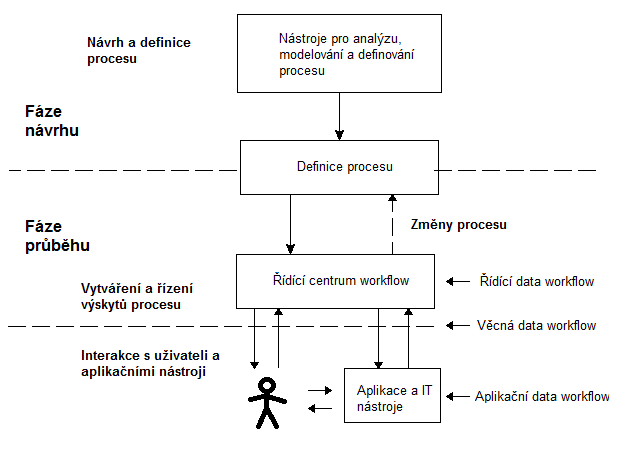
\includegraphics[width=340px]{images/faze_workflow.png}
\caption{Fáze workflow (převzato z \cite{wfmc})}
\end{figure}

\section{Workflow pro procesy pracující s vnitropodnikovými dokumenty}

Z pohledu charakteru procesů řadíme workflow pro procesy pracující s dokumenty do administrativních workflow. Většinou jsou to již procesy ustálené, dobře strukturované a tyto procesy jsou využívány většinou uživatelů systému. Z hlediska technologické infrastruktury jsou to systémy založené na dokumentech. Z hlediska orientace procesů patří do procesů orientovaných na sebe, jsou pro něj totiž typické vlastnosti jako předpověditelnost, strukturovanost, stálý postupu a je aktivován dokumenty.






\section{BPMN}
Buisiness Process Model And Notation (BPMN) je standard pro modelování podnikových procesů, jehož výstupem bývá grafické znázornění podnikových procesů v podobě procesních diagramů. \cite{bpmn} Jazyk BPMN také pomáhá sjednocovat významy základních pojmů používaných v této oblasti procesního řízení. 

Hlavním účelem BPMN je podporovat procesní řízení. Pro tuto funkci poskytuje notaci, která je jednoduchá, srozumitelná a intuitivní i pro netechnické pracovníky a zároveň dostatečná i pro vyjádření komplexních procesů. Přináší tedy standardizovaný zápis ve srozumitelné podobě pro všechny zainteresované osoby v organizacích.

Poslední verze BPMN 2.0 byla vydána v lednu 2011 a klade si za cíl být jedinou notací pro tvorbu modelů podnikových procesů. Proto mezi základními rysy jsou:
\begin{itemize}
\item snaha vytvořit jednotný konzistentní jazyk sjednocením definice podnikových procesů BPMN,
\item možnost vytvořit nezávislý nebo integrovaný model,
\item podpora a možnost výměny odlišných pohledů na procesní model tak, že je možno se v procesu zaměřit na slabá místa,
\item poskytnout xml schémata sloužící pro transformaci modelů.
\end{itemize}

Objekty jazyka BPMN jsou děleny do těchto základních kategorií. Tokové objekty, spojovací objekty, plavecké dráhy a artefakty. \cite{12}

\subsection{Tokové objekty}
Bývají označovány jako hlavní grafické prvky definující firemní procesy a dále se dělí.

\begin{itemize}
\item Události představují děje či události, ke kterým dochází v průběhu procesu.
\item Aktivity vyjadřují činnosti, které se odehrávají uvnitř procesu. Ty se dále dělí úlohy a podprocesy.
\item Brány jsou využívány pro zobrazení větvení a slučování toků a procesů, kdy je potřeba zohlednit různé podmínky. Dále jsou děleny na exkluzivní, inkluzivní a paralelní.
\end{itemize}

\begin{figure}[htp]
\centering

\includegraphics[width=210px]{images/tokove_objekty.png}
\caption{Tokové objekty}
\end{figure}


\subsection{Spojovací objekty}
Spojové objekty slouží ke spojování tokových objektů. Dělí se na sekvenční tok, tok zpráv a asociaci.

\begin{itemize}
\item Sekvenční tok znázorňuje posloupnost procesních toků v bazénu nebo podprocesu. Zdrojem a cílem je vždy nějaký tokový objekt. 
\item Tok zpráv označuje zprávy proudící přes hranice bazénů.
\item Asociace se používá pro připojení artefaktů nebo textu k tokovým objektům.
\end{itemize}

\begin{figure}[htp]
\centering
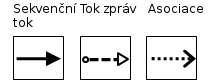
\includegraphics[width=210px]{images/spojovaci_objekty.png}
\caption{Spojovací objekty}
\end{figure}


\subsection{Plavecké dráhy}
Plavecké dráhy, někdy nazývané kontexty, slouží k organizování a kategorizaci činností. Rozlišují se typy: bazén a dráha.

\begin{itemize}
\item Bazén odděluje různé části popisované organizace.
\item Dráhy jsou součástí bazénu a používají se ke kategorizaci činností v rámci bazénu.
\end{itemize}

\begin{figure}[htp]
\centering
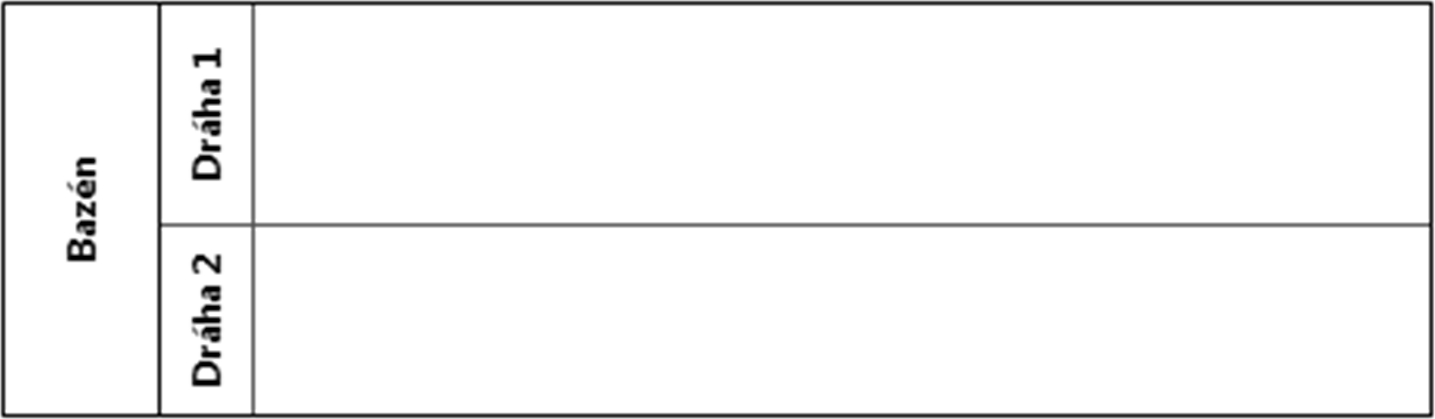
\includegraphics[width=340px]{images/bazen.png}
\caption{Bazén}
\end{figure}

\subsection{Artefakty}
Artefakty umožňují přidávat další informace do modelu a tím rozšiřují dostupné elementy v BPMN. Tím mohou zvyšovat informační hodnotu modelu. Existují tyto artefakty: datové objekty, skupiny a anotace.

\begin{itemize}
\item Datové objekty reprezentují nezbytná data pro vykonání dané činnosti.
\item Skupiny jsou využívány pro seskupení různých aktivit.
\item Anotace dodávají modelu srozumitelnost a přehlednost.
\end{itemize}

\begin{figure}[htp]
\centering

\includegraphics[width=340px,height=70px]{images/artefakty.png}
\caption{Artefakty}
\end{figure}



\chapter{Analýza a návrh aplikace}

Výstupem této diplomové práce je grafický editor pro návrh workflow, který bude pracovat v základní notaci BPMN a bude kompatibilní se standardním workflow systémem Kaleo, který je součástí Liferay Portal CE. V této kapitole nejprve popíši webový designer, který je využívaný pro jiný workflow systém Activiti, pak bude popsán Kaleo Designer, který je dodávaný v komerční verzi portálu Liferay Portal EE. Na závěr kapitoly bude provedena analýza požadavků na vytvářený systém.

\section{Activiti workflow}
Prvním používaným workflow systémem, který je možno použít v Liferay portálu je Activiti. Activiti se prezentuje jako jednoduché workflow, podporující standard BPMN 2. Tento projekt je šířen jako open-source pod licencí Apache license. Tento systém obsahuje několik nástrojů, které tvoří celou platformu Activiti a jsou to Activiti Engine, Activiti Modeler, Activiiti Designer, Activiti Explorer, Activiti Cycle a Activiti REST.

Pro tvorbu workflow je možné využít nástroje Activiti Modeler a Activiti Designer. Activiti Designer je plugin do vývojového prostředí Eclipse. Výsledkem této diplomové práce má být webová aplikace pro tvorbu workflow a proto tento nástroj není vhodný pro srovnání. 

Dalším nástrojem, který umožňuje vytvářet workflow je  Activiti Modeler \autoref{fig:activiti_modeler}. Je to open source webový nástroj pro modelování procesů. V počáteční fázi byl vyvíjen společností KIS BPM, nyní je již vyvíjen jako součást projektu Activiti. Hlavní cílem této aplikace je podporovat všechny BPMN elementy a rozšíření podporované Activiti Engine. 

\begin{figure}[htp]
\centering
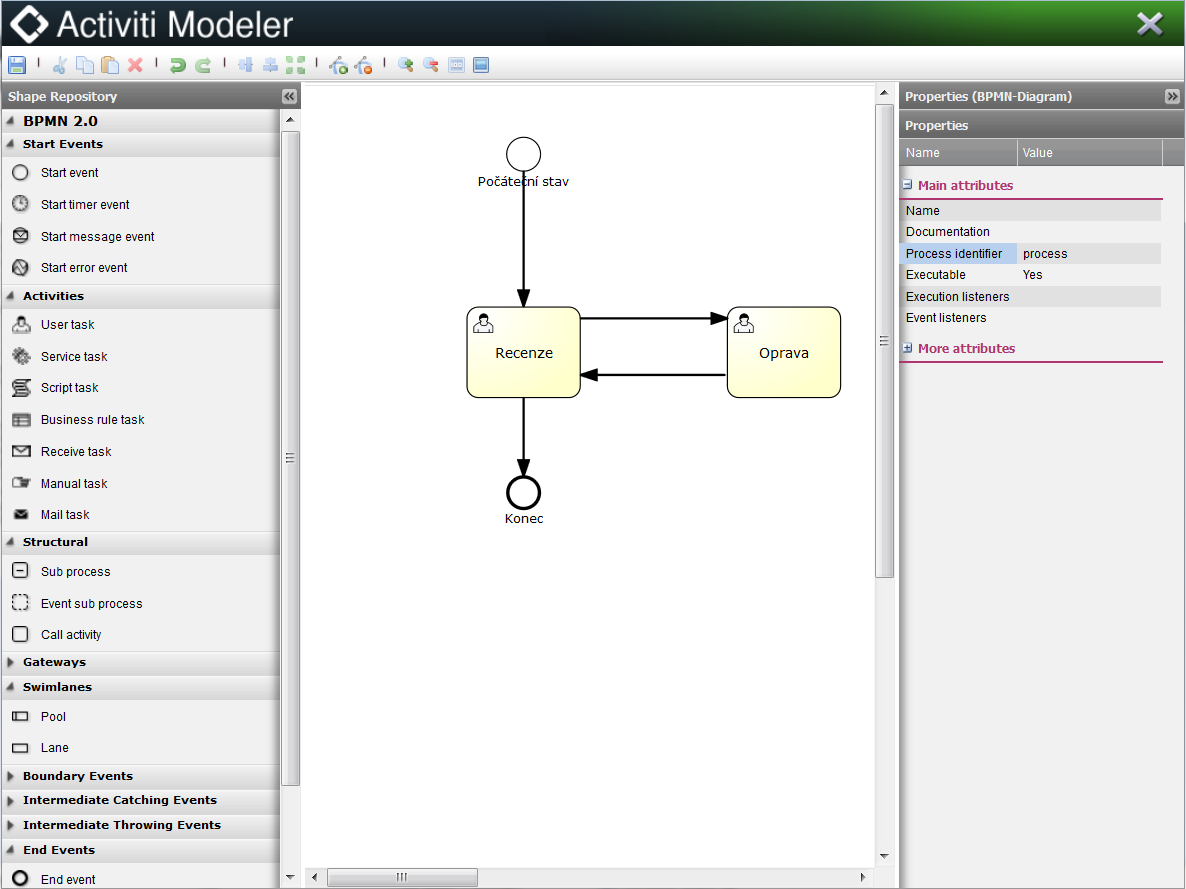
\includegraphics[width=340px]{images/activiti_modeler.png}
\caption{Activiti modeler}
\label{fig:activiti_modeler}
\end{figure}

Celá aplikace se skládá ze čtyř základních panelů. V prvním horní vodorovném panelu jsou uloženy všechny tlačítka, které reprezentují všechny akce, které je možné při modelování využít. Panel vlevo slouží jako paleta dostupných BPMN elementů. Na plátno, což je prostřední panel, se vkládají pomocí metody táhni a pusť. Poslední panel, umístěný vpravo, slouží pro úpravy vlastností jednotlivých entit či vlastností celého workflow.

\section{Kaleo designer v Liferay EE}
Kaleo designer je součástí portálu Liferay EE a je integrován přímo v portálu a je dostupný z control panelu. Je možné ho rozdělit na dvě hlavní části: seznam dostupných workflow v portálu a samotný grafický designer . V dalším popisu se zaměřím pouze na grafický designer, jehož detail můžeme vidět zde: \autoref{fig:kaleo_designer}.

\begin{figure}[htp]
\centering
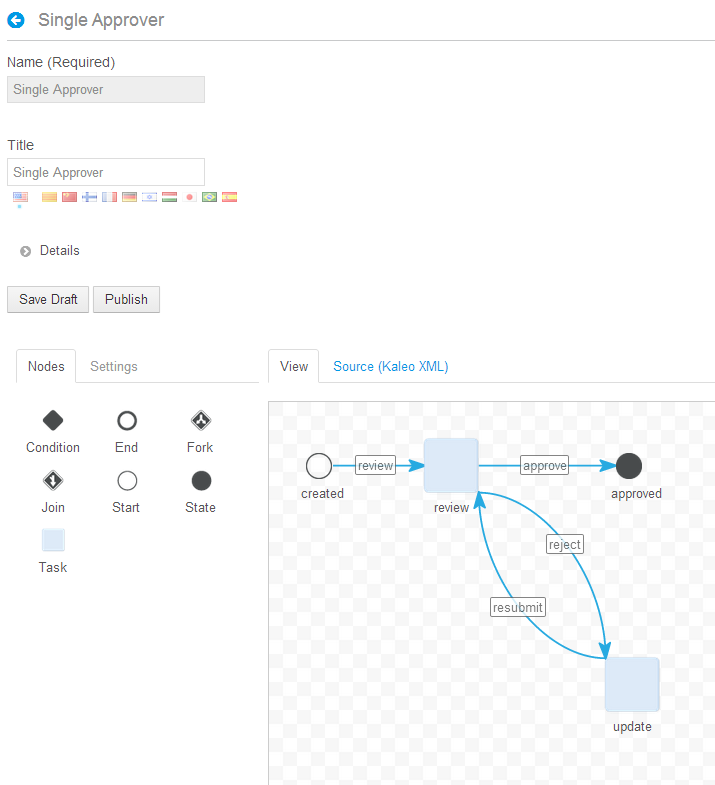
\includegraphics[width=340px]{images/kaleo_designer_detail.png}
\caption{Kaleo Designer detail}
\label{fig:kaleo_designer}
\end{figure}

Tento designer se také skládá ze tří základních panelů. V horním panelu jsou zobrazeny základní informace o workflow a také tlačítka pro dostupné akce s workflow. Pak se dělí na dva další panely. Levý panel slouží buď jako paleta dostupných elementů, nebo v případě vybrání některého elementu se v tomto panelu zobrazují podrobnosti a je možné je měnit pomocí vyskakovacích oken, ve kterých jsou dané formuláře. Těch vyskakovacích oken může být i více mohou se dokonce řetězit na sebe, což z uživatelského hlediska nepřijde úplně šťastné. Celkem jednoduše se můžeme dostat do situace, jenž je znázorněna zde: \autoref{fig:kaleo_designer_popup}.  Pravý panel obsahuje vlastní plátno nebo zdrojový kód v xml podle volby.

\begin{figure}[htp]
\centering
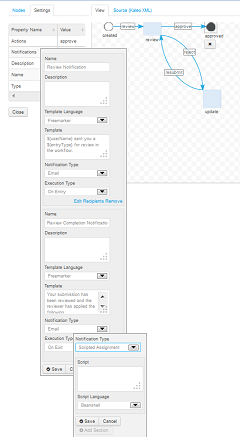
\includegraphics[width=240px, height=400px]{images/kaleo_designer_popup.png}
\caption{Řetězení vyskakovacích oken}
\label{fig:kaleo_designer_popup}
\end{figure}

\section{Požadavky na vytvářenou aplikaci}
Grafický editor pro tvorbu je velice speciální aplikace a při analýze požadavků jsem zjistil, že tento produkt má pouze jeden diagram užití. Hlavně z tohoto důvodu jsem zvolil analýzu v podobě seznamu požadavků.Tento způsob zápisu je také bližší zákazníkům, kterým bude následně tento produkt nabízen. Seznam těchto požadavků je uveden zde: \autoref{tab:seznam_pozadavku}.

\begin{table}[h]
\centering
\begin{tabular}{|p{5.5cm}|p{5.5cm}|}
\hline Kompatibilita s workflow systémem používaným v Liferay CE. & Výsledné XML schéma bude odpovídat požadovanému schématu workflow systémem Kaleo.  \\
\hline Editor umožní vytvářet a vkládát nové workflow definice. Také úmožní načítat již vložené definice v portálu.  & Editor bude napojen portálové API Liferay portálu. \\
\hline Editor umožní exportovat výsledné definice ve formátu XML.  & Bude možné exportovat vytvářené workflow definice do souboru ve formátu XML. \\
\hline Editor bude pracovat v základní notaci BPMN.  & Tento požadavek je omezen vlastnostmi workflow systému Kaleo, jenž umožňuje využít pouze některé prvky. \\
\hline  Editor bude v portálu přístupný pouze pro administrátory. & Editor bude umístěn v ovládacím panelu portálu v sekci konfigurace. \\
\hline Editor umožní uživateli vracet zpět provedené úpravy.  & Editor bude podporovat funkcionalitu zpět / vpřed. \\
\hline V editoru bude vytvářet i rozsáhlejší workflow definice.  & Editor bude umožňovat nastavit libovolnou velikost plátna. \\
\hline Uživatel bude mít možnost zkontrolovat správnost vytvářené workflow definice.  &  Editor bude umožňovat validaci vytvářené workflow definice. \\
\hline Aplikace by být přehledná a jednoduše použitelná.  & Bude omezeno použití vyskakovacích oken, které aplikace tohoto typu znepřehledňují. \\
\hline Editor bude umožňovat tvořit a upravovat skripty k akcím u jednotlivých elementů. & K těmto účelům bude k dispozici webový editor. \\
\hline K tvorbě skriptů bude mít uživatel k dispozici předpřipravené některé nejpoužívanější funkce.  &   Bude k dispozici seznam seznam vložitelných funkcí v jednom zvoleném skriptovacím jazyku. \\
\hline Výsledná aplikace by měla grafickým rozhraním zapadat do prostředí Liferay Portálu. & Pro tvorbu grafického rozhraní budou využity technologie, které jsou použity pro tvorbu grafického rozhraní portálu.\\

\hline
\end{tabular}
\caption{Seznam požadavků}
\label{tab:seznam_pozadavku}
\end{table}








\chapter{Realizace}
Aplikace není tvořena klasickou třívrstvou architekturou, protože není potřeba řešit perzistenci dat přímo v aplikaci. Výsledná workflow definice se buď vkládá přímo do portálu skrze portálové api nebo je možné výsledný XML soubor exportovat z aplikace. Proto se v následující části zaměřím hlavně na popis prezentační vrstvy a využití portálového api.

\section{Portletové MVC rámce}
Ve druhé kapitole byl představen životní cyklus portletu a hlavní koncepty vývoje portletů v Javě. Při vývoji podle portletové specifikace se portlet vytváří rozšířením třídy  \verb|GenericPortlet| a pomocí action a render metod, které obsahují navigační a validační logiku a zároveň se starají o zpracování akcí a generování obsahu. S přibývajícím množstvím funkcí se pak tato třída stává nepřehlednou a špatně udržovatelnou. Tento problém je možné řešit tím, že se rozdělí zodpovědnosti za zpracování požadavků do více specificky zaměřených komponent pomocí některého portletového rámce.

Portletové či webové rámce v sobě implementují osvědčené postupy a vzory pro zjednodušení vývoje. Pro vývoj portletů lze využít i ne přímo portletových rámců, například Struts nebo JSF, ale v takovémto případě je nutné použít takzvané portletové mosty, které řeší rozdíly mezi servletovým a portálovým životním cyklem. Toto řešení ale v sobě obsahuje vícefázový životní cyklus portletů a někdy to znesnadňuje využití plných možností portletové technologie. Portletový rámec navržený přímo pro vývoj portletů je rámec Spring MVC Portlet, který byl zvolen také pro vývoj této aplikace. Tento portletový rámec byl zejména proto, že je používaný ve firmě IBA CZ, pro kterou je tato práce řešena v rámci Sdružení průmyslových partnerů Fakulty informatiky.

\subsection{Spring Portlet MVC}
Rámec Spring Portlet MVC je založen na stejných konceptech, třídách a rozhraní jako Spring Web MVC framework \cite{spring-web-mvc}. Spring Portlet MVC je navržen pouze pro vývoj portletů a je možné pomocí něj vyvíjet portlety, které splňují portletové standardy JSR-168 i JSR-286. Také implementuje klasickou architekturu MVC. Ta se skládá z následujících částí. \cite{mvc} 

\begin{itemize}
\item Model (model) - je to doménově specifická reprezentace informací s nimiž aplikace pracuje.
\item View (pohled) - převádí data reprezentovaná modelem do podoby vhodné k prezentaci uživateli.
\item Controller (řadič) - reaguje na události a zajišťuje změny v modelu a pohledu.
\end{itemize}

Nejdůležitější roli v portletu má třída \verb|DispatcherPortlet|, která obstarává všechny příchozí požadavky, pro které volí vhodný řadič na zpracování požadavku. Každá instance dispečeru si udržuje vlastní aplikační kontext.


\section{Alloy UI framework}
Alloy je UI meta framework, který poskytuje konzistentní a jednoduché API pro vytváření webových aplikací na třech úrovní prohlížeče: struktura, styl a chování. Je založených na moderních technologiích CSS3, HTML5 a javascriptovém frameworku YUI3. \cite{alloy} V Liferay Portal od verze 6 nahradil tento framework dříve používané jQuery a staví se na něm grafické rozhraní Liferay portálu. 

\begin{figure}[htp]
\centering
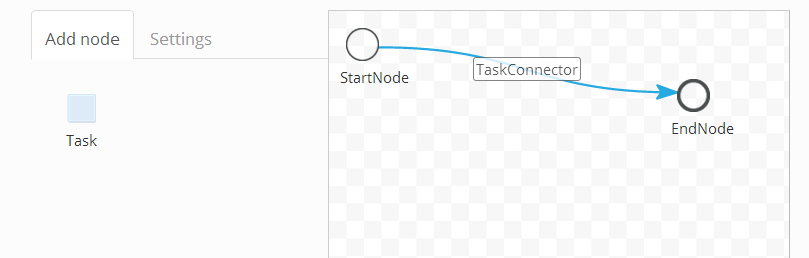
\includegraphics[width=340px, height=100px]{images/diagram_builder.png}
\caption{Alloy UI Diagram Builder komponenta}
\label{fig:diagram_builder}
\end{figure}

Pro tento framework jsem rozhodl z několika důvodů. Liferay Portal tento framework využívá pro tvorbu grafického rozhraní celého portálu a je proto již standardní součástí portálu, což jeho využití zjendnodušuje. Jeho použitím tedy dosáhnu stejného vzhledu jako je vzhled portálů, což je také jedním z požadavků kladených na tuto aplikaci. Dalším důvodem bylo, že Alloy UI poskytuje mnoho připravených komponent, které je možno využít. Z pohledu této práce je nejdůležitější komponentou Diagram Builder, viz. \autoref{fig:diagram_builder}. Pro potřeby aplikace byla tato komponenta rozšířena tak, aby ji bylo možné využít.


 Následuje úkazka kódu, na kterém je vidět, jak se takové rozšíření komponenty z Allyou UI provádí.

\begin{lstlisting}
AUI.add('my-diagram-builder', function(A, NAME) {

	var MyDiagramBuilder = A.Component
		.create({
			NAME : DIAGRAM_NAME,
				
			EXTENDS : A.DiagramBuilder,

			prototype : {
			}
	});

	A.MyDiagramBuilder = MyDiagramBuilder;

}, '2.0.0', {
	requires : [ ],
});

\end{lstlisting}
 

\section{JAXB}
Pro práci s daty ve formátu XML je využit nástroj JAXB (Java Architecture for XML Binding). Tento nástroj nabízí metody pro konverzi XML dat na Java objekt a naopak. Umožňuje také zápis a čtení XML z mnoho různých zdrojů.

Aby mohly být objekty určité třídy transformovány do XML dokumentů, tak musí obsahovat potřebné anotace. K základnímu vygenerování tříd podle XML schématu jsme využil kompilátor schémat, který je součástí JDK. Pak bylo ještě nutné upravit třídy.


\section{Portálové API}
Z portálového API jsou použity třídy \verb|WorkflowDefinitionManagerUtil| pro načítání, validaci a vkládání workflow definicí přímo do portálu. Dál jsou také využity entitní služby pro uživatele (\verb|UserLocalServiceUtil|) a role (\verb|RoleLocalServiceUtil|) v portálu, které slouží pro automatické doplňování ve formulářích.

\chapter{Testování aplikace}
Testováním je možné nazvat jakoukoliv aktivitu, která odhalí, že chování programu porušuje specifikaci. Nejčastěji bývá na testování nahlíženo jako na disciplínu, jejímž úkolem je ověřování kvality. Příkladem může být definice od Kanera \cite{kaner}: Softwarové testování je empirický technický výzkum kvality testovaného produktu nebo služby, prováděný za účelem poskytnutí těchto informací lidem, kterí mají zájem na dané věci. Na pojem kvalita produktu v tomto případě může být nahlíženo tak, že produkt má splnit požadavky určité potřeby, která stojí za jeho vznikem. Tedy kvalitní software je takový, který tyto potřeby uspokojuje.

Množina využitelných testů je velmi široká a proto je vždy nutné určit, jaké druhy testů budou použity, kdy a jak budou aplikovány. Webové aplikace patří do speciální skupiny softwaru a proto se zde používají určité druhy testování a ty je možné rozdělit do kategorií \cite{web-test}:  funkční testování, výkonnostní testování, testování použitelnosti, testování serverového rozhraní, testování kompatibility a testování bezpečnosti.

\section{Zvolené druhy testů}
Pro účely této aplikace jsem jako nejvhodnější zvolil funkční testování v kombinaci s testováním kompatability.

\subsection{Funkční testování}
Je to postup, kdy je ověřováno správné fungování aplikace nebo její části podle předem definovaného nebo očekávaného chování. Aplikace se při tomto testu prochází z pohledu uživatele a je tedy kontrolováno, zda reakce na uživatelovy akce a vstupy jsou správné a jestli aplikace podává správné výstupní informace a výsledky.

Zde je možné zahrnout kontrolu správnosti odkazování, ověřování funkčnosti formulářových prvků včetně validace vstupů a reakcí na chybný vstup. Mezi další patří také správná funkčnost JavaScript nebo AJAX částí aplikace.

\subsection{Testování kompatability}
Protože existují různé platformy spolu s rozmanitými prohlížeči, kde mohou být webové aplikace spouštěny, je testování kompatability velmi důležité. Je tedy vždy vhodné otestovat aplikaci na nejběžnějších kombinacích systémů, aby se tak zajistila správná funkčnost aplikace pro co nejširší okruh uživatelů.

\section{Příprava a průběh testů}
Aplikace workflow editor je určena pro tvorbu workflow definic v portálu Liferay. Jejím jediným uživatelem je administrátor portálu.Testování probíhalo podle předem určených určených testových scénářů na různých prostředí a v různých webových prohlížečích. Testové scénáře pokrývají všechny důležité funkce editoru a jsou to: vytvoření nového workflow, změna vloženého workflow, exportování workflow do souboru xml, přidání nového uzlu, přidání akce k uzlu, úprava akce u uzlu, přidání oznámení k uzlu, úprava oznámení u akce, u podmínky úprava scriptu, u úlohy úprava přiřazení, přidání časovače u uzlu, úprava časovače u uzlu. Níže jsou podrobně rozepsány scénaře na změnu workflow a úpravu akce u uzlu.

\subsection{Ukázkový testový scénář č.1 - Změna vloženého workflow}
\textbf{Vstupní podmínky:} Uživatel je v roli Administrátora (má tedy přístup k do kontrolního panelu), je přihlášený v portálu a v sekci kontrolní panel. Uživatel již vytvořil workflow a vložil ho do portálu na základě Vytvoření nového workflow.

\textbf{Scénář:}
\begin{enumerate}
\item Přechod na stránku s workflow editorem
\item Kliknutí na odkaz "Edit" na řádku workflow vytvořeného na základě Vytvoření nového workflow
\item Přidání nového stavu kliknutím na ikonu "Nový stav" (vizuální podoba - kruh)
\item Kliknutím do kreslící plochy (tímto se umístí nový stav)
\item Kliknutím na nově vytvořený stav 
\item Pak táhnutím nad cílový stav a kliknutím na něj se vytvoří nová vazba
\item Kliknutí na tlačítko "Uložit" pro uložení pozměněného workflow
\end{enumerate}


\section{Vyhodnocení testů}
Testy byly provedeny na různých prostředích a v různých prohlížečích. Bylo během nich nalezeno několik drobných chyb, které byly opraveny a odstranění chyb bylo znovu následně ověřeno.

\chapter{Dokumentace}



\chapter*{Závěr}
\addcontentsline{toc}{chapter}{Závěr}

%\printindex

\begin{thebibliography}{0}


\bibitem{gala}
GÁLA, L. et al. \textit{Podniková informatika}. 1. vyd. Praha: Grada Publishing, 2006. 

\bibitem{jsr-286}
\textit{JavaTM Portlet Specification}, The Java Community Process, dostupné na \url{http://www.jcp.org/en/jsr/detail?id=286} [cit. 2014-03-27].

\bibitem{cech}
ČECH, P. \textit {Přinos podnikových portálů pro management znalostí}, in Internet a konkurenceschopnost, Zlín, 2004.

\bibitem{enterprise-portal}
\textit{Enterprise portal}, Wikipedia, dostupné na \url{http://en.wikipedia.org/wiki/Enterprise_portal} [cit. 2014-03-27].

\bibitem{developer-guide}
\textit{Liferay Portal 6.2 Developer's Guide}, Liferay Inc., dostupné na \url{http://www.liferay.com/documentation/liferay-portal/6.2/development} [cit. 2014-04-02].

\bibitem{liferay-features}
\textit{Portal Features}, Liferay Inc., dostupné na \url{http://www.liferay.com/products/liferay-portal/features/portal} [cit. 2014-04-02].

\bibitem{portlets-in-action}
SARIN, Ashish. \textit{Portlets in action}, Shelter Island, NY: Manning, 2011.

\bibitem{wfmc}
\textit{Terminology \& Glossary}, Workflow Management Coalition, dostupné na \url{http://www.wfmc.org/standards/docs/TC-1011_term_glossary_v3.pdf} [cit. 2014-04-14].

\bibitem{workflow}
CARDA, A., KUNSTOVÁ, R. \textit {Workflow : Nástroj manažera pro řízení podnikových procesů}. 2. vyd. Praha: Grada Publishing, 2003.

\cite{bpmn}
\textit{Business Process Model and Notation (BPMN)}, Object Management Group, Inc., dostupné na \url{http://www.omg.org/spec/BPMN/2.0/} [cit. 2014-04-23]

\bibitem{spring-web-mvc}
Web MVC framework. \textit{Spring Framework Reference Documentation}, dostupné na \url{http://static.springsource.org/spring/docs/current/
spring-framework-reference/html/mvc.html} [cit. 2014-05-04]

\bibitem{mvc}
Model-view-controller. In: \textit{Wikipedia: the free encyclopedia} [online]. San Francisco (CA): Wikipedia Foundation, 2011

\bibitem{alloy}
\textit{http://alloyui.com/}

\bibitem{kaner}
ABRAN, A., MOORE, J.W. \textit{Guide to the Software Engineering Body of Knowledge} [online]. IEEE Computer Society, 2004 Version, dostupné na \url{http://www.inf.ed.ac.uk/teaching/courses/seoc/2006_2007/resources/SWEBOK_Guide_2004.pdf} [cit. 2014-05-08]

\bibitem{web-test}
VIJAY, S. \textit{Web Testing, Example Test cases} [online]., dostupné na \url{http://www.
softwaretestinghelp.com/web-testing-example-test-cases} [cit. 2014-05-08]

\end{thebibliography}


\newpage
\appendix
\chapter{Položky seznamu}


\end{document}